\documentclass[11pt,letterpaper]{article}

\usepackage[margin=1in]{geometry}
\usepackage{hyperref}
\usepackage{algorithm}
\usepackage{algorithmic}


%
\usepackage{hyperref,enumitem}
\hypersetup{
	colorlinks=true,
	citecolor = blue       %
}
\setlist{noitemsep,leftmargin=\parindent,topsep=2pt}
\setlist{noitemsep,topsep=2pt}
\usepackage{natbib}
\usepackage{url}            %
\usepackage{xspace}
%
\usepackage{graphicx}
\usepackage{amsmath,amssymb,amsthm}
\usepackage{booktabs} %
\usepackage{color}
\usepackage[font=small,labelfont=bf]{caption}
\usepackage{subcaption}
\usepackage{multirow}
\usepackage{authblk}
\renewcommand\Affilfont{\small}
\usepackage{comment}

\usepackage{tikz}
\usetikzlibrary{arrows}
\usetikzlibrary{shapes}
\usetikzlibrary{calc}

%
%

%
\usepackage{xcolor}
% Theorem-type environments

\newtheorem{theorem}{Theorem}
\newtheorem{lemma}[theorem]{Lemma}
\newtheorem{corollary}[theorem]{Corollary}
\newtheorem{proposition}[theorem]{Proposition}
\newtheorem{claim}[theorem]{Claim}
\newtheorem{observation}[theorem]{Observation}

\theoremstyle{definition}
\newtheorem{definition}[theorem]{Definition}
\newtheorem{remark}[theorem]{Remark}
\newtheorem{question}[theorem]{Question}
\newtheorem{conjecture}[theorem]{Conjecture}
\newtheorem{alg}[theorem]{Algorithm}
%\newtheorem{exercise}{}
\newtheorem{example}[theorem]{Example}

\definecolor{english}{rgb}{0.0, 0.5, 0.0}
\definecolor{brass}{rgb}{0.8, 0.58, 0.46}

\usepackage{tikz}
\usetikzlibrary{shapes}
\usetikzlibrary{calc}
\usetikzlibrary{decorations.pathreplacing}

\newcount\Comments 
\Comments=1
\newcommand{\kibitz}[2]{\ifnum\Comments=1{\color{#1}{#2}}\fi}
\newcommand{\zf}[1]{\kibitz{blue}{[ZF: #1]}}
\newcommand{\dcp}[1]{\kibitz{orange}{[DCP: #1]}}
\newcommand{\sdk}[1]{\kibitz{brass}{[SDK: #1]}}
\newcommand{\todo}[1]{\kibitz{blue}{[TODO: #1]}}
\newcommand{\sai}[1]{\kibitz{green}{[SAI: #1]}}

\newcount\CommentsA 
\CommentsA=1
\newcommand{\kibitzA}[2]{\ifnum\Comments=1{\color{#1}{#2}}\fi}
\newcommand{\dcpadd}[1]{{#1}}

%
\newenvironment{loneinnerlist}[1][\enskip\textbullet]%
{\vspace{-0.1\baselineskip}\begin{itemize}[#1]}
	{\end{itemize}\vspace{-0.1\baselineskip}}

\usepackage[utf8]{inputenc} % allow utf-8 input
\usepackage[T1]{fontenc}    % use 8-bit T1 fonts
\usepackage{hyperref}       % hyperlinks
\usepackage{url}            % simple URL typesetting
\usepackage{booktabs}       % professional-quality tables
\usepackage{amsfonts}       % blackboard math symbols
\usepackage{nicefrac}       % compact symbols for 1/2, etc.
\usepackage{microtype}      % microtypography
%\usepackage{natbib}
\usepackage{xcolor}         % colors
\usepackage[font=small]{caption}
\usepackage{subcaption}
\usepackage{enumitem}
\usepackage{amsmath,amssymb,amsthm}
\usepackage[algo2e, ruled]{algorithm2e} % For algorithms
\renewcommand{\algorithmcfname}{ALGORITHM}
\SetAlFnt{\small}
\SetAlCapFnt{\small}
\SetAlCapNameFnt{\small}
\SetAlCapHSkip{0pt}
\IncMargin{-\parindent}



\let\C\relax
\newcommand*{\C}{\mathbb{C}} 
\let\R\relax
\newcommand*{\R}{\mathbb{R}} 
\newcommand*{\Z}{\mathbb{Z}}
\newcommand*{\Zplus}{\mathbb{Z_+}}
\newcommand*{\Rplus}{\mathbb{R_+}}
\newcommand*{\PM}{\mathbb{PM}}
\newcommand*{\one}{\mathbbm{1}}
\newcommand*{\dotprod}[2]{\langle#1,#2\rangle}
\newcommand*{\prob}[1]{\mathbb{P}\left[#1\right]}

\newcommand*{\ex}[1]{\mathbb{E}\left[#1\right]}
\newcommand*{\norm}[1]{\|#1\|}
\newcommand*{\card}[1]{\lvert#1\rvert}
\newcommand*{\abs}[1]{\lvert#1\rvert}


\begin{document}
	
	
\title{Deep Learning for Two-Sided Matching\thanks{This work is supported in part through an AWS Machine Learning Research Award.}}

\author[a]{Sai Srivatsa Ravindranath}
\author[a]{Zhe Feng}
\author[b]{Shira Li}
\author[b]{Jonathan Ma}
\author[c]{Scott D.~Kominers}
\author[a]{David C.~Parkes}
%
%
%

\affil[a]{John A.~Paulson School of Engineering and Applied Sciences, Harvard University \authorcr \texttt{saisr,zhe\_feng,parkes@g.harvard.edu}}
\affil[b]{Harvard College \authorcr\texttt{shirali@alumni.harvard.edu, jonathan.q.ma@gmail.com}}
\affil[c]{Harvard Business School \authorcr \texttt{kominers@fas.harvard.edu}}

%\date{February 29, 2020}

\maketitle



\begin{abstract}
% \dcp{revised}\sdk{added a few tweaks} \sdk{Also, I think we could kill the first sentence of the abstract if we wanted to. Presumably it's redundant with the first couple sentences of the paper?}
%
%dcp edit Two-sided matching markets play a significant role in the modern life. And yet,  it is well-known that in two-sided matching, it is impossible to simultaneously achieve {\em stability} (such that no two parties prefer each other over their assigned matches) and {\em strategy-proofness} (such that there are no profitable misreports). At the same time, the necessary tradeoffs, and the degree to which one property can be  be achieved alongside  the other approximately, are not well understood. 
%
We initiate the use of a multi-layer neural network to model two-sided matching and to explore the design space between strategy-proofness and stability. It is well known that both properties cannot be achieved simultaneously but the 
efficient frontier in 
this design space is not understood.
We show empirically that it is possible to achieve a good compromise between stability and strategy-proofness---substantially better than that achievable through a convex combination of deferred acceptance  (stable and strategy-proof for only one side of the market) and randomized serial dictatorship  (strategy-proof but not stable).
\end{abstract}


\section{Introduction}
  
Two-sided matching markets, such as Uber, Airbnb,  stock markets, and dating apps, play a significant role in today's world. As a result, there is a tremendous and rising interest to design better mechanisms for two-sided matching. The seminal work of~Gale and Shapley~\cite{GS62} introduced a simple mechanism for stable matching in two-sided markets---\emph{Deferred-acceptance} (DA)---which has since has been applied in doctor-hospital matching~\cite{RothPeranson99}, school choice~\cite{abdulkadiroglu2003school,pathak2008leveling,APR2009}, and the matching of cadets to their branches of military service~\cite{sonmez2011matching,sonmez2011bidding}.
DA is \emph{stable}, i.e., no pair of agents mutually prefer each other to their DA partners. 
On the other hand, DA is not \emph{strategy-proof} (SP); that is, under fully general preferences, it is always possible that some agent can mis-report her preferences to obtain a better matching than she would receive under the DA mechanism.\footnote{As we discuss below, DA \textit{is} strategy-proof for agents on one side of the market, but not for agents on both sides of the market simultaneously.} 
%
Another well-known  mechanism, \emph{random serial dictatorship} (RSD), is SP but not stable.\footnote{\dcpadd{Indeed, RSD is typically studied for one-sided assignment problems rather than for two-sided matching mechanisms. For two-sided matching, not only is RSD unstable, but it can also fail to match participants in a way that is better than receiving no match at all. We adopt RSD as a benchmark in this paper---despite its flaws---because we are not aware of more suitable SP mechanisms for two-sided matching.}} More generally, it is well-known that it is impossible to achieve both stability and strategy-proofness in two-sided matching~\cite{DubinsFreeman1981,Roth82}. At the same time, there is little understanding of the nature of this tradeoff beyond point solutions such as DA and RSD---and we are not aware of any work that has attempted to map out the tradeoff
more generally. 
%


Inspired by the recent development of deep learning for optimal auction design~\cite{deep-auction19,curry2020certifying,STZ19,rahme2020permutationequivariant}, we initiate the study of multi-player neural networks to model two-sided matching.
%, based on the
%rich representation and approximation to nonlinear functions of deep neural networks. 
We show how to use machine learning to characterize the frontier curve of the tradeoff between stability and strategy-proofness.
%
The main challenges of applying neural networks to two-sided matching come from handling the ordinal preference inputs, and in identifying suitable differentiable surrogates for approximate strategy-proofness and stability.
 %
%To understand the tradeoff between stability and SP is not only of theoretical interest but can provide a useful matching mechanism in practice, for instance, \todo{any example about balancing SP and stability?} 
%

%We formulate suitable metrics along with a neural network architecture that outputs a distribution on  matchings. 
%dcp edit For this, we take the minimum of two appropriately defined softplus functions in the last layer of the neural network.
%to guarantee the feasibility of the randomized matching modeled by this neural network. 
%
%
For randomized matching mechanisms, the strongest SP concept is that of {\em ordinal strategy-proofness}. This aligns incentives with truthful reporting whatever the utility function of an agent. Ordinal SP is equivalent to a property of {\em first-order stochastic dominance} (FOSD)~\cite{Erdil14}, which means that agents have a weakly higher chance of getting their top-ranked choices when they report their preferences truthfully. %
%
Our metric for SP  quantifies the degree to which FOSD is violated. 
For this, we adopt an adversarial approach, seeking to augment the training data with suitable defeating mis-reports. We also provide a metric to quantify the degree to which stability is violated. 
We show that a loss function built from these quantities can be trained through SGD,
and illustrate the use of the framework 
to identify the stability-strategyproofness frontier. 
%
%
We run simulations to validate the efficiency of our approach, demonstrating for different preference distributions that our approach can strike much better trade-offs between stability and strategyproofness than the convex combination of DA and RSD. 

%To handle this difficulty, 

% \dcp{i sketched an outline for this section}

% \begin{itemize}
%     \item Importance of two-sided matching, including celebrated Gale Shapley and applications 
%     \item Lack of understanding about tradeoffs between approximate SP and approximate stability, potential importance of better understanding this
%     \item Role of deep learning (has been used for auctions, can it be used for two-sided matching), articulation of main challenges relative to auction design work 
%     \item Statement of novelty and summary of results 
% \end{itemize}

\paragraph{Related work.}
This work lies at the intersection of \emph{two-sided matching}~\cite{RothSotomayor1990} and the role of \emph{machine learning within economics}~\cite{Athey18}.
%
%\sdk{Could we  delete this next sentence and join the prior sentence with the next par?} We only present some closely related work here.
%
The matching mechanisms learned by our neural networks are randomized, approximately strategy-proof, and approximately stable. Budish et al.~\cite{BCKM13} and Mennle and Seuken~\cite{TimoSven16,mennle2021partial} discuss different notions of approximate strategy-proofness in the context of matching and allocation. In this work, we focus on ordinal SP and its analog of FOSD~\cite{Erdil14}. This is a strong and widely-used SP concept in the presence of ordinal preferences. 

Classic results of Dubins and Freedman~\cite{DubinsFreeman1981} and Roth~\cite{Roth82} show that it is impossible to achieve both stability and strategy-proofness in two-sided matching simultaneously---although strategy-proofness \textit{for one side of the market} is achieved by the Deferred Acceptance (DA) mechanism.\footnote{Alcalde and Barber\`{a}~\cite{alcalde1994top} also showed the impossibility of individually rational, Pareto efficient, and SP allocation rules. Alva and Manjunath~\cite{alva2020impossibility} extended this result to randomized matching contexts.} %Moreover, the preference restrictions required to get around failure of SP in the context of stable matching are quite strong \cite{}. 
Thus market designers have looked at mechanisms that relax one or both of these conditions. The \emph{Random serial dictatorship} (RSD) mechanism~\cite{AS98} is SP but typically fails to produce stable outcomes (and indeed, it may even fail to be individually rational).\footnote{The Top Trading Cycles (TTC) mechanism is likewise SP---but it effectively treats the market as one-sided, producing outcomes that do not reflect the other side's preferences.} On the other hand, Roth et al.~\cite{Roth93} study the polytope of stable matchings and provide a wide class of stable matchings beyond the well-known DA outcome. The \textit{stable improvement cycles} mechanism of Erdil and Ergin~\cite{erdil2008s}, meanwhile, achieves as much efficiency as possible on top of stability, but fails to be SP even for one side of the market. Finally, a series of results have shown that DA becomes SP for both sides of the market in certain large-market limit contexts; these results typically  also require additional, structural assumptions on market participants' preferences (see, e.g., \cite{immorlica2015incentives,kojima2009incentives,lee2016incentive}).

This work belongs to the emerging literature on \emph{machine learning for economic design}. Narasimhan et al.~\cite{NarasimhanParkes16a} utilize  support vector machines to search for good mechanisms among the weighted polytope mechanisms. Recently, many papers~\cite{deep-auction19, deep-budget, deep-facility, curry2020certifying,STZ19,rahme2020permutationequivariant} apply deep neural networks to optimal auction design and facility location problems. In this work, and inspired by the neural network architecture proposed by D\"{u}tting et al.~\cite{deep-auction19}, we use neural networks to model the design of two-sided matching markets. 
%and understand the tradeoff between stability and strategy-proofness. 

%
% 
%There are only few works  (e.g., \cite{TimoSven16}) seeking to understand the tradeoff between stability and strategy-proofness in two-sided matching, and these works do not characterize the frontier curve of the tradeoff.  
%


% \dcp{i sketched an outline for this section}

% \begin{itemize}
% \item Approximate SP (e.g., Seuken paper)
% \item FOSD and ordinal SP
% \item Rothblum et al understanding of the polytope of stable matchings, also my work with Hari in this regard 
% \item Anything known on fully SP mechanisms 
% \item Our work on deep learning for auctions (Note: I view the chapter as coming after this research paper, so I suggest we don't cite the chapter)
% \end{itemize}
\vspace{-5pt}
\section{Preliminaries}
\label{sec:prelim}
\vspace{-5pt}


% It is known to be impossible to achieve stability and strategy-proofness in two-sided matching markets. 
% In its place, economic theory gives
% well known, point solutions that offer different
% tradeoffs.  Deferred acceptance   provide
% stability, together with strategy-proofness on one side of the market. 
% Randomized serial dictatorship  provides 
% strategy-proofness, but without stability.

% In this section, we apply deep neural networks  to  the problem of learning
% matching mechanisms that make a  tradeoff between the degree
% of approximation to stability and the degree of approximation to strategy-proofness,
% adopting quantified measures of these approximations that are specialized
% to a particular preference distribution. This suggests
% new designs and  identifies gaps in
% our understanding from economic theory and 
% new targets for analytical study.

Let $W$ be a set of $n$ {\em workers} and $F$ a set of $m$ {\em firms}, and
suppose that each worker can be matched to at most one firm and each
firm to at most one worker.  A {\em matching} $\mu$ is a set of
(worker, firm) pairs, with each worker and firm participating in at
most one match. Let ${\mathcal B}$ denote the set of all
{\em matchings}. If a worker or firm remains unmatched, we say
that it is {\em matched to $\bot$}.
If $(w,f)\in \mu$, then $\mu$ matches $w$ to $f$, and
we write $\mu(w)=f$ and
$\mu(f)=w$. We write $(w,\bot)\in \mu$ (resp.~$(\bot,f)\in \mu$) to
denote that $w$ (resp.~$f$) is unmatched. 

Each worker has a {\em strict preference order} $\succ_w$ over the set
$\overline{F} = F\cup \{\bot\}$. Each firm has a strict preference order $\succ_f$
over the set $\overline{W} = W\cup \{\bot\}$.
%
Worker $w$ (firm $f$) prefers remaining
unmatched to being matched with a firm (worker) that is ranked below
$\bot$ (the agents ranked below $\bot$ are unacceptable).
If worker $w$ prefers firm $f$ to $f'$ then we represent this as
$f \succ_w f'$, and similarly for the preferences of a firm.  Let $P$ denote the set of all preference profiles,
with 
$\succ=(\succ_1,\ldots,\succ_n,\succ_{n+1},\succ_{n+m})\in P$  denoting the
preference  profile that comprises  all
workers and firms.

  A pair $(w,f)$ forms a {\em blocking pair for matching $\mu$} if $w$
  and $f$ prefer each other to their partners in $\mu$ (or $\bot$ in
  the case that either or both are unmatched).  A matching $\mu$ is {\em stable}
  if and only if there are no blocking pairs.
  A matching $\mu$ is {\em individually rational} (IR) if
  it is not blocked by any individual, i.e., there is no 
  worker or firm that finds its partner 
  unacceptable and prefers $\bot$.\footnote{Stability precludes empty matchings. For example, if  a matching
    $\mu$ leaves a worker $w$ and a firm $f$ unmatched, where $w$
    finds $f$ acceptable and $f$ finds $w$ acceptable, then $(w,f)$ is
    a blocking pair to $\mu$.}
  %
%
%   \begin{remark}
%     Stability precludes empty matchings. For example, if  a matching
%     $\mu$ leaves a worker $w$ and a firm $f$ unmatched, where $w$
%     finds $f$ acceptable and $f$ finds $w$ acceptable, then $(w,f)$ is
%     a blocking pair to $\mu$.
%     \end{remark}
    
\subsection{Randomized matchings}

We work with {\em randomized matching mechanisms} $g$ that map preference profiles $\succ$ 
   to distributions on matchings, denoted
  $g(\succ)\in \triangle({\mathcal B})$. 
  This provides for differentiable mechanisms.
  Here, 
  $\triangle({\mathcal B})$ denotes the probability simplex on the set
  of matchings.

We  write $r\in [0,1]^{(n+1)\times (m+1)}$ to define  
the {\em marginal probability} $r_{wf}\geq 0$ with which  worker $w$ is matched with firm $f$, for each $w\in \overline{W}$
and each firm $f\in \overline{F}$. We require $\sum_{f'\in \overline{F}} r_{wf'}= 1$ for all $w\in W$, 
and $\sum_{w'\in \overline{W}}r_{w'f}=1$ for all $f\in F$. For notational simplicity, we also write $g_{wf}(\succ)$ to denote the marginal probability of matching worker $w$ (or $\bot$) and firm $f$ (or $\bot$). 
%
\begin{theorem}[Birkhoff von-Neumann]
Given any randomized matching $r$, there exists a distribution on  matchings, $\Delta({\mathcal B})$,
with marginal probabilities equal to $r$.   
\end{theorem}

The following definition is standard~\cite{BCKM13} %\dcp{can we add a cite?}, 
and generalizes stability to randomized matchings.
%
\begin{definition}[Ex ante justified envy]
\label{def:envy}
A randomized matching $r$ causes {\em ex ante justified envy} if

(1) some worker $w$ prefers $f$ over some (fractionally) matched firm $f'$ (including $f'=\bot$) and firm $f$ prefers $w$ over some (fractionally) matched worker $w'$ (including $w'=\bot$) (``$w$ has envy towards $w'$" and   ``$f$ has envy towards  $f'$"), or

(2) some worker $w$ finds a (fractionally) matched $f'\in F$ unacceptable, i.e. $r_{wf'}>0$ and $\bot \succ_w f'$, or some firm $f$ finds a (fractionally)  matched $w'\in W$ unacceptable, i.e. $r_{w'f}>0$ and $\bot \succ_f w'$.
\end{definition}

\if 0
For example, if  worker $w$  prefers firm $f$ to some  $f'$, and  $f$ prefers  $w$ to some $w'$, then there
is envy when $f$ is matched to $w'$ with some probability ($w$ envies $w'$) and $w$ is matched to $f'$ with some probability ($f$ envies $f'$).
%
As another example, if worker $w$  prefers $f$ to $f'$, and $f$ prefer $w$ to $\bot$, then  there
is  envy when $w$ is matched to $f'$ with some probability and $f$ is unmatched  with some probability. %dcp edit for conciseness Here, 
% $f$ has envy towards $f'$ (since $f'$ sometimes matches with $w$) and $w$ has envy towards $\bot$ (since $\bot$ sometimes matches with $f$). 
 %This can also be similarly stated when $f'$ takes the role of $\bot$, or when both $w'$ and $f'$ take the role of $\bot$.
%
%There is also ex ante justified envy when some worker $w$ may prefer to be unmatched than its match, or some firm $f$ may prefer to be unmatched than its match.
\fi

%\sdk{Is there a reason why this definition doesn't incorporate IR as a part of stability?} \dcp{which defn? i think ex ante just envy does} 

A randomized matching $r$ is {\em ex ante stable} if and only if it does not cause any {\em ex ante} justified envy. Ex ante stability reduces to the standard concept of stability for a deterministic matching. 
%
%\zf{Remove one theorem}.
% \begin{theorem}
% For a deterministic matching, ex ante stability 
% is equivalent to stability. 
% \end{theorem}
% %
% \begin{proof}
% For a deterministic matching, there is  {\em ex ante justified envy} if and only if there is a blocking pair. The worker $w$ and firm $f$ with ex ante justified envy prefer each other over their respective matches, with $(w',f)$ and $(w,f')$ matched, and form a blocking pair.
% \end{proof}
%
Part~(2) of the definition of ex ante justified envy captures
the idea that a randomized matching $r$ 
should satisfy \emph{individually rationality} (IR). 
%
That is, for  any worker $w$, we should have $r_{wf'} = 0$ for all $f'\in F$ for which $\bot \succ_w f'$, and for any firm $f$, we should have $r_{w'f}$ for all $w'\in W$ for which $\bot \succ_f w'$. %In this paper, we consider a strong strategy-proofness for randomized matchings proposed by~\cite{},


To define  strategy-proofness, 
say that $u_w: \overline{F}\to \mathbb{R}$ is a {\em $\succ_w$-utility} for 
worker $w$ when  $u_w(f)>u_w(f')$ if and only if $f\succ_w f'$, for all $f, f'\in \overline{F}$. We similarly define a $\succ_f$-utility for firm $f$.
%
The following concept of ordinal SP is standard~\cite{Erdil14} % zf edit: \dcp{need cite}
and generalizes SP to randomized matchings.
%
\begin{definition}[Ordinal strategy-proofness]\label{def:ordinal-sp}
A randomized matching mechanism $g$ satisfies ordinal SP if and only if, for all agents  $i\in W\cup F$,  for any preference profile $\succ$, and any $\succ_i$-utility for agent $i$, 
then for all reports  $\succ'_i$, we have
\begin{align}
    \mathbf{E}_{\mu\sim g(\succ_i, \succ_{-i})}[u_i(\mu(i))] \geq \mathbf{E}_{\mu\sim g(\succ'_i, \succ_{-i})}[u_i(\mu(i))].
\end{align}
%
\end{definition}

By this definition, no worker or firm can improve its expected utility by misreporting their preference order, and for any   utility function consistent with their preference order.
%
For a deterministic mechanism,  ordinal SP reduces  to the  
requirement that no agent can improve its preference ranking for any misreport.
%, whatever the reports of others (and thus SP).

% \dcp{state as defn and then thm}

% This is equivalent to requiring that  the distribution on matchings for the true report 
% {\em first order stochastically dominates} (FOSD) the distribution for a misreport, 
% i.e., for worker $w$, and for each $f'\in \overline{F}$, we have
% %
% \begin{align}
% \sum_{f\in F: f\succ_w f'} g_{wf}(\succ_w, \succ_{-w}) & \geq \sum_{f\in F: f\succ_w f'} g_{wf}(\succ'_w, \succ_{-w}).
% \end{align}

Erdil~\cite{Erdil14} characterizes the following {\em first-order stochastic dominance condition} as equivalent to  ordinal SP (Definition~\ref{def:ordinal-sp}); this  condition provides a useful relaxation of SP for our learning framework.
 %
\begin{definition}[First Order Stochastic Dominance]\label{def:fosd-sp}
 A randomized matching mechanism $g$ has {\em first order stochastic dominance}  (FOSD) if and only if, the distribution on matchings for the true report 
{\em first order stochastically dominates} the distribution for a mis-report, 
e.g., for worker $w$, and for each $f'\in \overline{F}$ such that $f' \succ_{w} \bot$, and all reports of others $\succ_{-w}$, we have (and similarly for the roles of workers and firms transposed)
%
\begin{align}
\sum_{f\in F: f\succ_w f'} g_{wf}(\succ_w, \succ_{-w}) & \geq \sum_{f\in F: f\succ_w f'} g_{wf}(\succ'_w, \succ_{-w}).
\end{align}
\end{definition}

\dcpadd{Whether looking at its most preferred firm, its two most preferred firms, or so forth,  worker $w$ achieves a higher probability of matching on that firm or set of firms for its true report than for any mis-report, and whatever the reports of others.}

%\dcp{note, i'm calling this just FOSD. I think we can retain SP for ordinal SP}

\begin{theorem}[\cite{Erdil14}]\label{thm:fosd}
A two-sided matching  mechanism is ordinal  SP if and only if it satisfies FOSD.
\end{theorem}

% \todo{Add a short interpretation?}
 
% \dcp{ introduce relaxed version of FOSD for $r < 1$ if we use it}

% We also find it useful to work with a weaker kind  of strategy-proofness. 
% %
% \begin{definition}[Convex strategy-proofness]
% A randomized matching mechanism $g$ is {\em convex strategy-proof} if and only if, for all agents (including workers and firms), $i\in W\cup F$, and   any preference profile $\succ$, there exists  a valid utility function $u_i$ for $\succ_i$, s.t. for all reports $\succ'_i$, we have %$\mathbb{E}_{g_i(\succ_i, \succ_{-i})}[u_i] \geq \mathbb{E}_{g_i(\succ'_i, \succ_{-i})}[u_i]$.
% \begin{align}
%     \mathbf{E}_{\mu\sim g(\succ_i, \succ_{-i})}[u_i(\mu(i))] \geq \mathbf{E}_{\mu\sim g(\succ'_i, \succ_{-i})}[u_i(\mu(i))].
% \end{align}
% \end{definition}

%  For a randomized matching,  convex strategy-proofness
%  may only align incentives for a particular utility function rather than every utility function.
% %
% %This property reduces to full strategy-proofness for a deterministic matching mechanism.
% %
% \begin{theorem}
% \label{thm:11}
% For a deterministic matching, convex strategy-proofness is equivalent to full strategy-proofness.
% \end{theorem}
% \begin{proof}
% Consider a deterministic matching mechanism $g$, for any agent $i\in W\cup F$ and any preference order $\succ_i$, for all preference profiles $\succ_{-i}$ and all misreports $\succ'_i$, let $\mu \sim g(\succ_i, \succ_{_i})$ and $\mu' \sim g(\succ'_i, \succ_{_i})$. Since $g$ is deterministic, $\mu$ and $\mu'$ are both unique. Then convex strategy-proofness of mechanism $g$ implies $\mu(i) \succ_i \mu'(i)$. Therefore, for any valid utility function $u_i$ for $\succ_i$, we have 
% $u_i(\mu(i)) \geq u_i(\mu'(i))$, which implies full strategy-proofness.% \zf{A bit long, better to shorten it.}
% \end{proof}

% For this reason, we will also be interested to understand the amount of randomization that is used in
% the learned mechanisms.


%\dcp{prob want to add a brief note here that we tend to produce deterministic mechanisms in practice }

 %
% Convex strategy-proofness is convenient to work with  when 
% developing the machine learning pipeline for
% two-sided matching. 
 %see Step 2. in Section~\ref{sec:matching-methodology}.
  
  \if 0
  In the case of a randomized mechanism, it is
  convenient to let $\omega$ denote the random coin flips, internal to
  the mechanism.  Given this, let $M(\succ; \omega)\in \mathcal{M}$
  denote the realized matching for input profile $\succ$.
%
  \begin{definition}[stability]
    A {\em mechanism is stable} if, for all preference profiles
    $\succ\in P$, and  all random draws $\omega$ of the mechanism,
    we have that matching
    $M(\succ;\omega)$ is stable. 
  \end{definition}
\fi


  
%  Given preference profile $\succ$, and a modified preference order,
%  denoted $\succ'_x$, reported by some worker or firm $x\in W\cup F$,
%%  let $\succ'$ denote the preference profile that is the same as
 % $\succ$ except for participant $x$, when it takes on $\succ_x'$.
  
  \if 0
   %x   
  \begin{definition}[strategy-proofness]
  A {\em mechanism is strategy-proof} if, for all preference profiles
  $\succ\in P$, and all random draws $\omega$ of the mechanism, we have
  %
  \begin{itemize}
    \item For every worker $w$, and every preference order $\succ_w'
     \  \neq\ \succ_w$,  then  $\mu(w)\succ_w\mu'(w)$ for
      $\mu=M(\succ;\omega)$ and $\mu'=M(\succ';\omega)$.
      %
      \item For every firm $f$, and every preference order $\succ_f'
   \   \neq \ \succ_f$,  then  $\mu(f)\succ_f\mu'(f)$ for
      $\mu=M(\succ;\omega)$ and $\mu'=M(\succ';\omega)$.
    \end{itemize}
    \end{definition}
    
    \fi

\subsection{Deferred Acceptance and RSD}

% \dcp{consider stating roth 82 thm about impossibility of stability and SP.check with scott what's know about generalization of thm to randomized mechanisms}

%As already noted, in two-sided matching, it is impossible to achieve both stability and strategy-proofness simultaneously. Thus 

In this section, we consider two benchmark mechanisms: the stable but not SP \emph{deferred-acceptance} (DA) mechanism---which is a deterministic mechanism---and the SP but not stable \emph{randomized serial dictatorship} (RSD) mechanism.
%
DA mechanisms are stable and ordinal SP for the proposing side of the market,
but they are not ordinal SP for both sides. 
% zf-edits
% \dcp{i edited following to handle truncations . pls check}\zf{looks good}
%
\begin{definition}[Deferred-acceptance (DA)]\label{def:DA}
In worker-proposing deferred-acceptance (firm-proposing is defined analogously), each worker $w$ maintains a list of acceptable firms ($f\succ_w \bot$) for which it has not had a proposal rejected (``remaining firms").
Repeat the following process until all proposals are accepted:
\begin{itemize}[leftmargin=*]
\item $\forall w\in W$: $w$ proposes to its best acceptable, remaining firm.
%
\item $\forall f\in F$: $f$ tentatively accepts its best proposal (if any), 
and rejects the rest.
%
\item $\forall w\in W$: If $w$ is rejected by firm $f$, it updates its list of acceptable firms to remove $f$.
\end{itemize}
\end{definition}

\begin{theorem}[see \cite{RothSotomayor1990}]
DA is stable, but not FOSD strategy-proof.
\end{theorem}
%In addition, we consider another simple mechanism.

%
\begin{definition}[Randomized serial dictatorship (RSD)]\label{def:RSD}
Sample a {\em priority order} $\pi$ on the set $W\cup F$ uniformly at
random, such that $\pi_1, \pi_2, \ldots, \pi_{m+n}$ is a
permutation on $W\cup F$ in decreasing order of
priority. Proceed as follows:
%
\begin{itemize}[leftmargin=*]
\item Initialize matching $\mu$ to the empty matching. 
\item In round $k=1, \ldots, m+n$:
\begin{itemize}
\item If $\pi_k\in W\cup F$ is not yet matched in $\mu$, then add to
matching $\mu$ the match between $\pi_k$ and its most preferred,
unmatched agent, or $\bot$ if all
remaining possibilities are unacceptable to $\pi_k$.
\end{itemize}
%\item Modify $\mu$, replacing any  matches $(w,f)\in \mu$
%  that are unacceptable to either $w$ or $f$
%  with  $(w,\bot)$ and
%  $(\bot,f)$. x
% dcp: as per my slack, not SP  with this step
\end{itemize}
%
\end{definition}

\begin{theorem}
RSD satisfies FOSD---and thus is ordinal SP by Theorem~\ref{thm:fosd}---but is not stable. 
\end{theorem}
% \zf{Remove the proof and example.}
% \dcp{can put in place a simple discussion to explain}
%% ZF-edits: remove the proof and the example.
\begin{proof}
For ordinal SP, 
%it suffices to establish that, for any valid utility,  there is no useful manipulation 
%whatever the priority order $\pi$ (and thus also in expectation over priority orders).
consider agent  $i$ in some position $k$ in the order. The agent's reported preference order has no effect on the choices of preceding agents, whether workers or firms (and even in regard to whether agent $i$ itself is selected by an agent on the other side of the market). Reporting its true preference order ensures that it is matched with 
its most preferred agent of those remaining, in the event that it remains unmatched by the time position $k$ is reached. % This is best, whatever its (valid) utility function. 
Example~\ref{ex:1} in Appendix~\ref{app:rsd-unstable} shows that RSD is not stable.
\end{proof}
% \todo{@Sai: move the commented example to Appendix.}

% \begin{example}
% \label{ex:1}
% Consider 3 workers and 3 firms with the following preference orders:
% \begin{align*}
%     w_1: f_2, f_3, f_1, \bot \quad f_1: w_1, w_2, w_3, \bot\\
%     w_2: f_2, f_1, f_3, \bot \quad f_2: w_2, w_3, w_1, \bot\\
%     w_3: f_1, f_3, f_2, \bot \quad f_3: w_3, w_1, w_2, \bot
% \end{align*}
% The  matching found by worker-proposing DA is $(w_1, f_3), (w_2, f_2), (w_3, f_1)$. This is a stable matching. If $f_1$ truncates and misreports its preference as $f_1: w_1, w_2, \bot, w_3$, the matching found is $(w_1, f_1), (w_2, f_2), (w_3, f_3)$. Firm $f_1$ is matched with a more preferred worker, and hence the mechanism is not strategy-proof.
% %
% Now consider a particular realization of the matching under RSD. For  priority order $\pi = (w_1, f_1, w_2,$ $f_2, w_3, f_3)$, the matching   is $(w_1, f_2), (w_2, f_1), (w_3, f_3)$.
% RSD is strategy-proof. However, we can see that $(w_2, f_2)$ is a blocking pair, and hence it is not stable.
% \end{example}

\section{Two-Sided Matching as a Learning Problem}\label{sec:learning}

In this section, we show how to use deep learning to model a two-sided matching mechanism and then formulate two-sided matching as a learning problem. %Finally we provide the training procedure for our neural networks.

\subsection{Neural Network Architecture}\label{sec:matching-methodology}

We use a neural network to represent a two-sided matching  mechanism.  We write $\theta\in \mathbb{R}^d$ to denote the parameters of the network ($d$ parameters). Let $g^\theta: P\to \triangle({\mathcal B})$ denote the corresponding  mechanism.
%
%
This network provides a differentiable representation of a distribution on matchings for each preference profile.

We use  a feed-forward neural network with $R = 4$ fully-connected hidden layers,   $J = 256$ units in each layer,  leaky ReLU activations, and a fully-connected output layer. 
See Figure~\ref{fig:gen-net-2}.
%Empirically, we have found that 
%good performance in these two-sided matching settings 
%requires larger networks than in the smaller auction settings and better performance with leaky ReLU  than tanh activations.
%\dcp{consider a FN to define leaky-ReLU and motivate their use }
%\zf{Do we want to mention the parameters here or leave it to experimental section?}
%\dcp{experimental}
We represent a preference order at the input to the neural network by adopting an evenly spaced utility function.  \dcpadd{This is simply a representation choice and still allows the adoption of an FOSD-based metric for the study of approximately SP mechanisms.}
%
Given a preference  profile $\succ$, the preference representation for a worker $w\in W$ and a firm $f\in F$ is given by $p^\succ_w = (p_{w1}^\succ, \ldots, p_{wm}^\succ)$ and $q^\succ_f= (q_{1f}^\succ, \ldots, q_{nf}^\succ)$ respectively.  We also 
define $p^{\succ}_{w\bot} = 0$ and $q^\succ_{\bot f}=0$. For example:
%

$\bullet$ For a preference order $\succ$ with $w_1: f_1, f_2, \bot, f_3$, we have $p^\succ_{w_1}=(\frac{2}{3},\frac{1}{3},-\frac{1}{3})$. 
 
 
 $\bullet$ For a preference order $\succ$ with $w_1: f_1, f_2, \bot, f_3, f_4$, we have $p^\succ_{w_1}=(\frac{2}{4},\frac{1}{4},-\frac{1}{4},-\frac{2}{4})$.
 
 
 $\bullet$ For a preference order $\succ$ with $f_1: w_2, w_1, w_3$, we have $q^\succ_{f_1}=(\frac{2}{3},1,\frac{1}{3})$.


%\zf{Do we need to write a mathematical formula for $p$ and $q$.} 

%\dcp{following defn of p and q can go to appendix if we need the space} 
For some worker $w$'s utility for firm $j$ and some firm $f$'s utility for worker $i$, and with $\mathbf{1}(E)$ to indicate the indicator function for event $E$,
we have:
%
\[
\!\! p_{wj}^\succ \!=\!  \frac{1}{m}\!\left(\! \mathbf{1}_{ j \succ_{w} \bot} + \sum_{j'=1}^{m} (\mathbf{1}_{j \succ_{w} j'} - \mathbf{1}_{\bot \succ_{w} j'}) \!\right);
\ \ 
%\label{eq:p}
q_{if}^\succ\! =\!  \frac{1}{n} \!\left( \mathbf{1}_{i \succ_{f} \bot} + \sum_{i'=1}^{n} (\mathbf{1}_{i \succ_{f} i'} - \mathbf{1}_{\bot \succ_{f} i})\!\right).
%\!, \quad \mbox{for $i\in W$} \label{eq:q}
\]

\if 0
For worker $w$ and firm $j$, the quantity  $p^\succ_{wj}$ 
for a firm $j$ that is acceptable to $w$ is  $1/m$  times the count of  one plus the number of firms $j'$  for which $j\succ_w j' $ and $j'\succ_w \bot$ ($j'$ is acceptable).
%
The quantity  $p^\succ_{wj}$ for worker $w$ and  a firm $j$ that is unacceptable to $w$ is  $1/m$  times the negated count of the number of 
 firms $j'$ for which it is not the case that $j\succ_w j'$ (this includes when $j'$ is the same as $j$), and where $\bot\succ_w j'$ and thus $j'$ is unacceptable (the indicators inside the parentheses are both zero for acceptable firms $j'$, and both one for unacceptable firms $j'$ that are less preferred than $j$).
 %
 \fi
 

The vector $(p_{11}^\succ, \ldots, p_{nm}^\succ, q_{11}^\succ, \ldots, q_{nm}^\succ)$ constitutes the input to the  network ($2\times n \times m$ numbers).
%


%
\begin{figure}[t]
%\input{regret-net-multi-buyer-unit-demand.tex}
\centering
%\documentclass{article}
%\usepackage{tikz}
%\usetikzlibrary{shapes}
%\usetikzlibrary{calc}
%
%\begin{document}
%
%%%%MULTI-BUYER, MULTI-ITEM
%\begin{figure}
%\centering
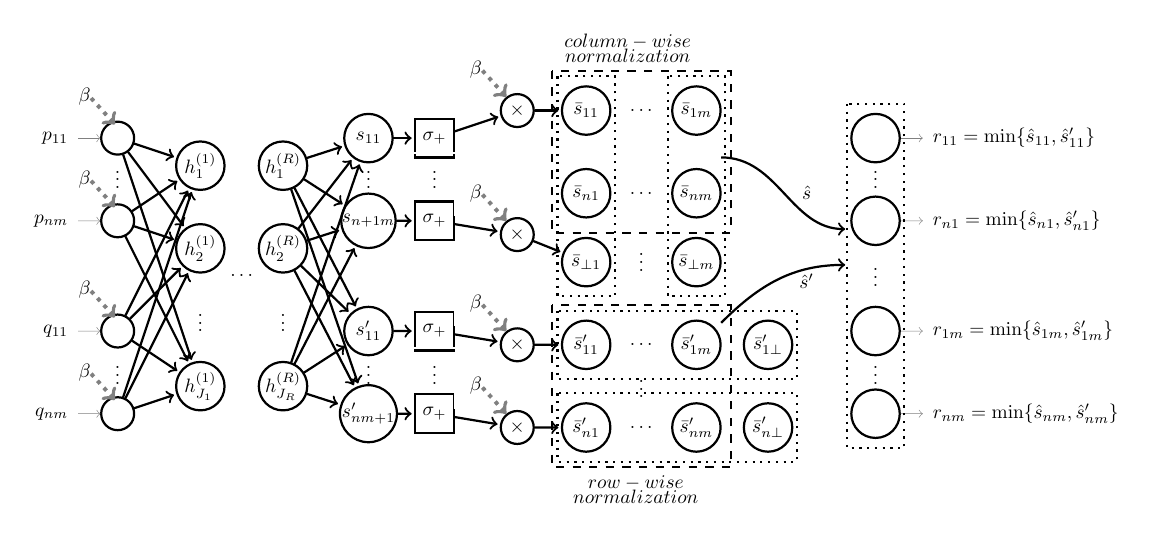
\begin{tikzpicture}[scale=0.7, transform shape, shorten >=1pt,->,draw=black!100, node distance=\layersep, thick]
    \tikzstyle{input text}=[draw=white,minimum size=22pt,inner sep=0pt]
    \tikzstyle{input neuron}=[circle,draw=black!100,minimum size=17pt,inner sep=0pt,thick]
    \tikzstyle{hidden neuron}=[circle,draw=black!100,minimum size=25pt,inner sep=0pt,thick]
    \tikzstyle{hidden text}=[draw=white,minimum size=22pt,inner sep=0pt,thick]
    \tikzstyle{unit}=[circle,draw=black!100,minimum size=25pt,inner sep=0pt,thick]
    \tikzstyle{squnit}=[draw=black!100,minimum size=20pt,inner sep=0pt,thick]
     
    \def\x{0.25}
    % Draw the input layer nodes
    \node[input text] (I-10) at (0,-0.65) {$\vdots$};
    \node[input text] (I-20) at (0,-4.2) {$\vdots$};
    \node[input neuron, pin={[pin edge={<-}]left:$p_{11}$}] (I-1) at (0,0) {};
    \node[input neuron, pin={[pin edge={<-}]left:$p_{nm}$}] (I-2) at (0,-1.5) {};
    \node[input neuron, pin={[pin edge={<-}]left:$q_{11}$}] (I-3) at (0,-3.5) {};
	\node[input neuron, pin={[pin edge={<-}]left:$q_{nm}$}] (I-4) at (0,-5) {};  
	
	\node[hidden text] (temp-1) at (-0.6, 0.75) {$\beta$};
    \node[hidden text] (temp-1) at (-0.6, -0.75) {$\beta$};
    \node[hidden text] (temp-1) at (-0.6, -2.75) {$\beta$};
    \node[hidden text] (temp-1) at (-0.6, -4.25) {$\beta$};
    
	\draw[<-,solid,line width=0.5mm,dotted,color=gray] (-0.05, 0.25)  -- (-0.55, 0.75 + 0.05); 
	\draw[<-,solid,line width=0.5mm,dotted,color=gray] (-0.05, -1.25)  -- (-0.55, -0.75 + 0.05); 
	\draw[<-,solid,line width=0.5mm,dotted,color=gray] (-0.05, -3.25)  -- (-0.55, -2.75 + 0.05); 
	\draw[<-,solid,line width=0.5mm,dotted,color=gray] (-0.05, -4.75)  -- (-0.55, -4.25 + 0.05);
	
	
	\node[input text] (temp-1111) at (2.25, -2.5) {$\ldots$};

    % Draw the hidden layer nodes
    \path node[hidden text] (H-0) at (1.5,-3.25) {\vdots};
    \path node[hidden neuron] (H-1) at (1.5,-0.5) {$h^{(1)}_1$};
    \path node[hidden neuron] (H-2) at (1.5,-2) {$h^{(1)}_2$};
    \path node[hidden neuron] (H-3) at (1.5,-4.5) {$h^{(1)}_{J_1}$};
    
    
    \foreach \dest in {1,...,3}
    	\foreach \src in {1,...,4}
			\path (I-\src) edge (H-\dest); 		
    
    % Draw the hidden layer nodes
    \path node[hidden text] (J-0) at (3,-3.25) {\vdots};
    \path node[hidden neuron] (J-1) at (3,-0.5) {$h^{(R)}_1$};
    \path node[hidden neuron] (J-2) at (3,-2) {$h^{(R)}_2$};
    \path node[hidden neuron] (J-3) at (3,-4.5) {$h^{(R)}_{J_{R}}$};
    
    
    \node[input text] (S-10) at (4.55,-0.65) {$\vdots$};
    \node[input text] (S-20) at (4.55,-4.2) {$\vdots$};
    \path node[unit] (S-1) at (4.55,-0) {$s_{11}$};
    \path node[unit] (S-2) at (4.55,-1.5) {$s_{n+1m}$};
    \path node[unit] (S-3) at (4.55,-3.5) {$s'_{11}$};
    \path node[unit] (S-4) at (4.55,-5.0) {$s'_{nm+1}$};
    
    
    
     \foreach \src in {1,...,3}
		\foreach \dest in {1,...,4}
			\path (J-\src) edge (S-\dest); 
    

    \path node[squnit] (T-1) at (5.75,-0) {$\sigma_+$};
    \path node[squnit] (T-2) at (5.75,-1.5) {$\sigma_+$};
    \path node[squnit] (T-3) at (5.75,-3.5) {$\sigma_+$};
    \path node[squnit] (T-4) at (5.75,-5.0) {$\sigma_+$};
    
    \node[input text] (T-10) at (5.75,-0.65) {$\vdots$};
    \node[input text] (T-20) at (5.75,-4.2) {$\vdots$};
    
    \foreach \src in {1,...,4}
			\path (S-\src) edge (T-\src); 
			
	\path node[input neuron] (U-1) at (\x +7.0,0.5-0) {$\times$};
    \path node[input neuron] (U-2) at (\x +7.0,-0.25-1.5) {$\times$};
    \path node[input neuron] (U-3) at (\x +7.0,-0.25-3.5) {$\times$};
    \path node[input neuron] (U-4) at (\x +7.0,-0.25-5.0) {$\times$};
    
    \node[hidden text] (temp-1) at (6.5, 1.25) {$\beta$};
    \node[hidden text] (temp-1) at (6.5, -1.0) {$\beta$};
    \node[hidden text] (temp-1) at (6.5, -3.0) {$\beta$};
    \node[hidden text] (temp-1) at (6.5, -4.5) {$\beta$};
    
	\draw[<-,solid,line width=0.5mm,dotted,color=gray] (7.05, 0.75)  -- (6.55, 1.25 + 0.05); 
	\draw[<-,solid,line width=0.5mm,dotted,color=gray] (7.05, -1.5)  -- (6.55, -1.0 + 0.05); 
	\draw[<-,solid,line width=0.5mm,dotted,color=gray] (7.05, -3.5)  -- (6.55, -3.0 + 0.05); 
	\draw[<-,solid,line width=0.5mm,dotted,color=gray] (7.05, -5.0)  -- (6.55, -4.5 + 0.05);
    
     \foreach \src in {1,...,4}
			\path (T-\src) edge (U-\src);
    
    \path node[hidden neuron] (V-1) at (\x +8.25,0.5-0) {$\bar s_{11}$};
    \path node[hidden neuron] (V-2) at (\x +8.25,0.5-1.5) {$\bar s_{n1}$};
    \path node[hidden neuron] (V-25) at (\x +8.25,0.5-2.75) {$\bar s_{\bot 1}$};
    \path node[hidden neuron] (V-3) at (\x +8.25,0.25-4.0) {$\bar s'_{11}$};
    \path node[hidden neuron] (V-4) at (\x +8.25,0.25-5.5) {$\bar s'_{n1}$};
    %\node[input text] (V-10) at (\x +8.25,-0.65) {$\vdots$};
    %\node[input text] (V-10) at (\x +8.25,-4.2) {$\vdots$};
    
    
	\path (U-1) edge (V-1);
	\path (U-2) edge (V-25);
	\path (U-3) edge (V-3);
	\path (U-4) edge (V-4);
	
			
	\path node[hidden neuron] (W-1) at (\x +10.25,0.5-0) {$\bar s_{1m}$};
    \path node[hidden neuron] (W-2) at (\x +10.25,0.5-1.5) {$\bar s_{nm}$};
    \path node[hidden neuron] (W-25) at (\x +10.25,0.5-2.75) {$\bar s_{\bot m}$};
    \path node[hidden neuron] (W-3) at (\x +10.25,0.25-4.0) {$\bar s'_{1m}$};
    \path node[hidden neuron] (W-4) at (\x +10.25,0.25-5.5) {$\bar s'_{nm}$};
    \path node[hidden neuron] (W-35) at (\x +11.55,0.25-4.0) {$\bar s'_{1\bot}$};
    \path node[hidden neuron] (W-45) at (\x +11.55,0.25-5.5) {$\bar s'_{n\bot}$};
    
    
    %\node[input text] (W-100) at (\x +10.25,0.5-0.65) {$\vdots$};
    %\node[input text] (W-200) at (\x +10.25,0.5-4.2) {$\vdots$};
    
    \node[input text] (W-11) at (\x +9.25,0.5-0) {$\ldots$};
    \node[input text] (W-12) at (\x +9.25,0.5-1.5) {$\ldots$};
    \node[input text] (W-13) at (\x +9.25,-0.25-3.5) {$\ldots$};
    \node[input text] (W-14) at (\x +9.25,-0.25-5) {$\ldots$};
    \node[input text] (W-15) at (\x +9.25,-1.5-0.65) {$\vdots$};
    \node[input text] (W-16) at (\x +9.25,-0.25-4.2) {$\vdots$};
    
    
    
    \node[input text] (temp-111) at (\x +12.5+1.0,-0.65) {$\vdots$};
    \node[input text] (temp-222) at (\x +12.5+1.0,-2.42) {$\vdots$};
    \node[input text] (temp-333) at (\x +12.5+1.0,-4.2) {$\vdots$};
    \path node[unit, pin={[pin edge={->}]right:$r_{11} = \min\{\hat{s}_{11},\hat{s}'_{11}\}$}] (X-1) at (\x +12.5+1.0,-0) {};
    \path node[unit, pin={[pin edge={->}]right:$r_{n1} = \min\{\hat{s}_{n1},\hat{s}'_{n1}\}$}] (X-2) at (\x +12.5+1.0,-1.5) {};
    \path node[unit, pin={[pin edge={->}]right:$r_{1m} = \min\{\hat{s}_{1m},\hat{s}'_{1m}\}$}] (X-3) at (\x +12.5+1.0,-3.5) {};
    \path node[unit, pin={[pin edge={->}]right:$r_{nm} = \min\{\hat{s}_{nm},\hat{s}'_{nm}\}$}] (X-4) at (\x +12.5+1.0,-5) {};
   
			
	\draw[thick,dotted] ($(X-1.north west)+(-0.2,0.3)$)  rectangle ($(X-4.south east)+(0.2,-0.3)$);
	\draw[thick,dotted] ($(W-1.north west)+(-0.2,0.3)$)  rectangle ($(W-25.south east)+(0.2,-0.3)$);
	\draw[thick,dotted] ($(V-1.north west)+(-0.2,0.3)$)  rectangle ($(V-25.south east)+(0.2,-0.3)$);
	\draw[thick,dotted] ($(V-3.north west)+(-0.2,0.3)$)  rectangle ($(W-35.south east)+(0.2,-0.3)$);
	\draw[thick,dotted] ($(V-4.north west)+(-0.2,0.3)$)  rectangle ($(W-45.south east)+(0.2,-0.3)$);
	
	\draw[thick,dashed] ($(V-1.north west)+(-0.3,0.4)$)  rectangle ($(W-2.south east)+(0.3,-0.4)$);
	\draw[thick,dashed] ($(V-3.north west)+(-0.3,0.4)$)  rectangle ($(W-4.south east)+(0.3,-0.4)$);
	
	\node at  ($(W-16.west) + (0.3, -0.05-1.75)$) {$row-wise$};
	\node at  ($(W-16.west) + (0.3, -0.05-2.0)$) {$normalization$};
	
	\node at  ($(V-1.east) + (0.3, +1.25)$) {$column-wise$};
	\node at  ($(V-1.east) + (0.3, +1.0)$) {$normalization$};
	
	%\node[hidden text] (temp-111) at (\x +11.5,-1.1) {$\hat{s}$};
    %\node[hidden text] (temp-222) at (\x +11.5,-3.95) {$\hat{s}'$};
    
    %\path[draw=black,solid,line width=1mm,fill=black] (\x +11,-1.0) -- (\x +12,-2);
	%\path[draw=black,solid,line width=1mm,fill=black] (\x +11,-4.0) -- (\x +12,-3);
	
	\coordinate (LL1) at (\x +10.70,-0.35);
    \coordinate (LL2) at (\x +12.5+0.5,-1.65);
    
    \coordinate (LL3) at (\x +10.70,-3.35);
    \coordinate (LL4) at (\x +12.5+0.5,-2.30);
    
    \node[hidden text] (LL-5) at (12.5, -1.0) {$\hat{s}$};
    \node[hidden text] (LL-5) at (12.5, -2.6) {$\hat{s}'$};


	\draw [thick,black] (LL1) to[out=0,in=180] (LL2);
	\draw [thick,black] (LL3) to[out=45,in=180] (LL4);
    
      
   

\end{tikzpicture}
%\end{figure}
%
%\end{document}
\caption{Matching network $g$ for a set of $n$ workers and $m$ firms. Given inputs $p, q \in \mathbb{R}^{n \times m}$ the matching network is a feed-forward  network with $R$ hidden layers that uses softplus activation to generate non-negative scores and normalization to compute the  randomized matching. We additionally generate a Boolean mask matrix, $\beta$, and multiply it with the score matrix before normalization to ensure IR by making the probability of matches that are unacceptable  zero.}
\label{fig:gen-net-2}
\vspace{-10pt}
\end{figure}


%\zf{Sai: Add a description that the mask method guarantees IR.}

The output of the network is a vector $r \in [0, 1]^{n \times m}$ with  $\sum_{j = 1}^{m} r_{wj} \leq 1$ and 
$\sum_{i = 1}^{n} r_{if} \leq 1$  for every every $w \in [n]$ and $f \in [m]$. 
This describes the marginal probabilities in a randomized matching for this input profile. %
%\dcp{ **FIXED** sai, check following for dimensions... I think we needed one more dimension to handle dummy?}
The network first outputs two sets of scores $s\in \R^{(n + 1) \times m}$ and $s' \in \R^{n \times (m + 1)}$.
%
We apply the {\em softplus function} (denoted by $\sigma_+$) element-wise to these scores, where $\sigma_+(x) = \ln (1 + e^{x})$. 
To ensure IR, we first construct a Boolean mask variable $\beta_{wf}$, which is zero only when the match is unacceptable to one or both the worker and firm, i.e., when $\bot \succ_{w} f$ or $\bot \succ_{f} w$. We set $\beta_{n+1, f} = 1$ for $f \in F$ and $\beta_{w, m+1} = 1$ for $w \in W$. We multiply the scores $s$ and $s'$ element-wise with the corresponding Boolean mask variable to compute $\bar s \in \R_{\geq 0}^{(n + 1) \times m}$ and $\bar s' \in \R_{\geq 0}^{n \times (m + 1)}$.

For each $w \in \overline{W}$, we have $\bar s_{wf} = \beta_{wf} \ln (1 + e^{s_{wf}})$, for all $f\in F$. For each  $f \in \overline{F}$, we have
   $\bar s'_{wf} = \beta_{wf} \ln (1 + e^{s'_{wf}})$,  for all $w \in W$.
%
We  normalize $\bar s$ along the rows and  $\bar s'$ along the columns to obtain {\em normalized scores}, $\hat s$ and $\hat s'$ respectively. The  match probability $r_{wf}$, for worker $w \in W$ and firm $f \in F$, is computed as the minimum of the normalized scores:
%
$r_{wf} = \min\left(\frac{\bar s_{wf}}{\sum_{f' \in \overline{F}} \bar s_{wf'}},  
\frac{\bar s'_{wf}}{\sum_{w' \in \overline{W}} \bar s'_{w'f}} \right)$.
%
We have $r_{wf} = 0$ whenever $\beta_{wf} = 0$, ensuring that every matching 
in the support of the distribution will be IR. 
%zf-edit
Based on our construction, the allocation matrix $r$ is always (weakly) doubly stochastic \footnote{This is a more general definition for doubly stochastic than is typical. Doubly stochastic is usually defined on a
square matrix with the sum of rows and the sum of columns equal to 1.}. Budish et al.,~\cite{BCKM13} shows any (weakly) doubly stochastic matrix can be decomposed to a convex combination of 0-1 (weakly) doubly stochastic matrices. 
%\zf{@David: is this OK?}

% \zf-edit: \dcp{cite paper that shows how to take a partially, double stoch matrix and get to a fully double stoch matrix}
%\dcp{sai, will need to point here to method in appendix to go to a fully doubly stochastic matrix, and from there to using Birkhoff von-Neumann to get well defined distribution over matchings including $\bot$} 

\subsection{Formulation as a Learning Problem}

We formulate a {\em loss function} $\mathcal L$ that  is defined on training data
$D=\{\succ^{(1)},\ldots,\succ^{(L)}\}$, with each preference
profile $\succ$ in D sampled i.i.d.~from a distribution  on profiles. 
%
We allow for {\em correlated preferences}; e.g, 
workers may tend to agree that one of the firms is preferable to
one of the other firms, and similarly for firms. 
%
The loss function  captures a tradeoff between the
degree with which stability  and ordinal SP is violated.
%
\if 0
\dcp{(1) Define stability violation (which should follow as a relaxation of no justified envy), and will be in expectation over type profiles}
    
\dcp{(2) Define SP violation (should follow as a relaxation of convex-SP), and will be in expectation over type profiles}
    
\dcp{(3) Note that zero stability violation => stable up to measure zero , and zero SP violation => convex SP up to measure zero} \zf{Done}
    
    \fi
    %
Recall that $g^\theta(\succ) \in [0, 1]^{n \times m}$ denotes the randomized matching. %given by a mechanism $g$
%for a preference order profile $\succ$. 
%
We write $g^\theta_{w\bot}(\succ) = 1 - \sum_{f = 1}^{m} g^\theta_{wf}(\succ)$ and $g^\theta_{\bot f}{(\succ)} = 1 - \sum_{w=1}^{n} g^\theta_{wf}(\succ)$ to denote the probability of worker $w$ and firm $f$ being unmatched, respectively. 

\paragraph{Stability Violation.}
For worker $w$ and firm $f$, we define the {\em   stability violation }
at profile $\succ$ as
%
\begin{align}
 \!\!\!\!       \mathit{stv}_{wf}(g^\theta, \succ) &\!=\! 
\left(\sum_{w' = 1}^{n} g^\theta_{w'f}(\succ)\cdot\max\{q_{wf}^\succ - q_{w'f}^\succ, 0\} + g^\theta_{\bot f}(\succ) \cdot\max\{q_{wf}^\succ, 0\}\!\!\right) \\ \notag
&  \times \! \left(\sum_{f' = 1}^{m} g^\theta_{wf'}(\succ)\cdot \max\{p_{wf}^\succ - p_{wf'}^\succ,0\} + g^\theta_{w\bot}(\succ) \cdot\max\{p_{wf}^\succ, 0\}\!\!\right)  
% &+\sum_{w'=1}^n g_{w'f}(\succ)\max\{-q^\succ_{w'f},0\}\\ \notag
% &
% +\sum_{f'=1}^m g_{wf'}(\succ)\max\{-p^\succ_{wf'},0\}
\end{align}
 % We can check that $\mathit{stv}_{wf}(g,\succ)>0$ if and only if there is ex ante justified envy for this worker and firm. 
  %
  
  
This captures the first kind of {\em ex ante} justified envy in Definition~\ref{def:envy}, which is in regard to fractionally matched partners. We can omit the second kind of {\em ex ante} justified envy because the learned mechanisms satisfy IR through the use of the Boolean mask matrix (and thus have no violations of the second kind).



%\dcp{don't we divide this by something?}
The  average 
 stability violation  (or just stability violation) of  mechanism $g^\theta$ on  profile $\succ$
 is 
$\mathit{stv}(g^\theta, \succ) =  \frac{1}{2}\left(\frac{1}{m}  +\frac{1}{n}\right)\sum_{w = 1}^{n}\sum_{f = 1}^m \mathit{stv}_{wf}{(g^\theta, \succ)}.$
%\dcp{consider dividing this by $n\times m$ to make it comparable to the per-agent regret calculation}
We can define the expected stability violation $\mathit{STV}(g^\theta)=\mathbb{E}_{\succ} \mathit{stv}(g^\theta,\succ)$. We also write  $\mathit{stv}(g^\theta)$ to denote the  average stability violation  of a mechanism $g^\theta$ on the training data.
%
%, over all  preference  profiles in
%the training data, is $\mathit{stv}(g^\theta) = \frac{1}{L}\sum_{\ell = 1}^{L} %\mathit{stv}(g^\theta, \succ^{(\ell)})$.
%
%A randomized matching is ex ante stable if and only if $\mathit{stv}(g, \succ)=0$.
%
%\dcp{I edited this to speak to ex ante stability. pls check}
%
\begin{theorem}\label{thm:stability-violation}
A  randomized matching mechanism $g^\theta$ is ex ante stable up to zero-measure events 
if and only if  $\mathit{STV}(g^\theta)=0$.  
\end{theorem}   
\begin{proof}
Since $\mathit{stv}(g^\theta, \succ)\geq 0$ then $\mathit{STV}(g^\theta)=\mathbb{E}_{\succ} \mathit{stv}(g^\theta,\succ)=0$ if and only if 
$\mathit{stv}(g^\theta, \succ)= 0$ except on zero measure events. 
Moreover, $\mathit{stv}(g^\theta, \succ)= 0$ implies $\mathit{stv}_{wf}(g^\theta,\succ)=0$ for all $w\in W$, all $f\in F$.  This is equivalent to no justified envy.
%
For firm $f$, this means $\forall w'\neq w$, $q^\succ_{wf} \leq  q^\succ_{w'f}$ if $g^\theta_{w'f} > 0$ and $q\succ_{wf} \leq 0$ if $g^\theta_{\bot f} > 0$. Then there is no justified envy for firm $f$. Analogously, there is no justified envy for worker $w$. If $g^\theta$ is ex ante stable, it trivially implies $STV(g^\theta)=0$ by definition.
% that  there is no justified envy \dcp{complete; SAI, would rather write the theorem like this... can you fill in?}
%
\if 0

$\mathit{stv}(g^\theta,\succ)>0$, and so $\mathit{stv}_{wf}(g^\theta,\succ)>0$ for some $w\in W$ and $f\in F$. Since the terms in the summation are all non-negative, there exists a $w'$ (or $\bot$) and $f'$ (or $\bot$) for which $g^\theta_{w'f}(\succ)>0$ and $g^\theta_{wf'}>0$, and where $p^\succ_{wf}-p^\succ_{wf'}>0$, i.e., $f \succ_w f'$, and $q^\succ_{wf}-q^\succ_{w'f}>0$, i.e., $w \succ_f w'$ (note $p^\succ_{w\bot} = q^\succ_{\bot f}=0$). Moreover, if the matching is ex ante stable, then $\mathit{stv}_{wf}(g^\theta, \succ) = 0$ for any pair $(w, f)$, by  definition. This establishes the equivalence in the definitions.

\fi
%
\if 0

We prove by contradiction. For any fixed preference profile $\succ$, suppose a randomized matching $r$ by mechanism $g$ causes ex ante justified envy of worker $w$ toward a worker (or $\bot$) $w'$ with $w \succ_f w'$ for some firm $f$ if $r_{wf'}(\succ) > 0$ for some $f \succ_w f'$ ($f'\in \overline{F}$) and $r_{w'f}(\succ) > 0$. For any valid utility functions, $u_w$ for $w$ and $u_f$ for $f$, % $(p^\succ, q^\succ)$
associated with the preference profiles $\succ$, we have
\begin{align*}
\mathit{stv}(g, \succ) &\geq \mathit{stv}_{wf}(g, \succ) \notag \\&\geq \left(r_{w'f}(\succ) \cdot (u_f(w) - u_{f}(w'))\right)  \times \left(r_{wf'}(\succ)\cdot(u_{w}(f) - u_{w}(f')) \right) \notag \\ &> 0.
\end{align*}
\fi
\end{proof}


%
%% ZF-edits: remove the example for now, we can move it to Appendix if needed.
% \begin{example}
% Consider the preference  profile in Example~\ref{ex:1}. We have: 
% \[ 
% p^\succ = \left( \begin{array}{ccc}
% \frac{1}{3} & 1  & \frac{2}{3} \\
% \frac{2}{3} & 1 & \frac{1}{3} \\
% 1 & \frac{1}{3} & \frac{2}{3} 
% \end{array} \right)
% %
% ~\text{and}~q^\succ = 
% \left( \begin{array}{ccc}
% 1           & \frac{1}{3} &  \frac{2}{3}\\
% \frac{2}{3} & 1           &  \frac{1}{3} \\
% \frac{1}{3} & \frac{2}{3} &  1
% \end{array} \right)
% \]

% Consider the matching given by a particular priority order in the RSD mechanism:
% \[ 
% g(\succ)^{\mathrm{RSD}} = \left( \begin{array}{ccc}
% 0 & 1  & 0 \\
% 1 & 0 & 0  \\
% 0 & 0 & 1 
% \end{array} \right). \]

% We have,
% \[ \mathit{stv}_{wf}(g_{\mathrm{RSD}}, \succ) = \begin{cases} 
%           \frac{1}{9}, & \mbox{if $(w,f) = (2, 2)$} \\
%          0 & \mbox{otherwise}. \\
%       \end{cases}
%     \]
    
% We see that the stability violation is non-zero where there is a blocking pair, and zero otherwise.
% \end{example}

    
% \begin{definition}[Weakly SD-Strategyproofness]
%  A randomized matching mechanism $g$ is weakly SD-strategyproof if for all agents $i\in N$, all preference profiles $(\succ_i,\succ_{-i})$, and all misreports $\succ'_i$, the allocation vector $g_i(\succ_i, \succ_{-i})$ stochastically dominates $g_i(\succ'_i, \succ_{-i})$ at $\succ_i$ whenever the two allocation vectors are comparable by stochastic dominance at $\succ_i$.
% \end{definition}


%
%\dcp{sai, add here the approx to FOSD and a thm to say it's ordinal SP if and only if zero }
% \dcp{depending on where we end up, also define the $r$ version of approx SP and the fixed utility version}

\paragraph{Regret.}
We turn now to quantifying the degree of 
approximation to ordinal SP.
For a valuation profile $\succ \ \in P$ and a mechanism $g^\theta$, the {\em regret} to a worker (firm) for submitting their truthful preference, for some valid utility function,  is the maximum amount by which the worker (firm) could increase their expected utility through a mis-report, fixing the reports of others.
%
Let $\succ_{-i}=(\succ_1,\ldots,\succ_{i-1},\succ_{i+1},\ldots,\succ_{n + m})$.
%
%\zf{Sai: redefine the regret based on FOSD definition.}
%
The regret to worker $w$ at preference order $\succ$ is 
\begin{eqnarray}\label{eq:regret-worker}
\mathrm{regret}_w(g^\theta, \succ) = \max_{\succ'_{w} \in P} \left( \max_{f' \in F, f' \succ_{w} \bot} \sum_{f\in F: f\succ_w f'} g^\theta_{wf}(\succ'_w, \succ_{-w}) -  g^\theta_{wf}(\succ_w, \succ_{-w})\right).
\end{eqnarray}
%
The regret to a firm $f$ at preference order $\succ$ is
%
\begin{eqnarray}\label{eq:regret-firm}
\mathrm{regret}_f(g^\theta, \succ) =  \max_{\succ'_{f} \in P} \left( \max_{w' \in W, w' \succ_{f} \bot} \sum_{w\in W: w\succ_f w'} g^\theta_{wf}(\succ'_f, \succ_{-f}) -  g^\theta_{wf}(\succ_f, \succ_{-f}) \right). 
\end{eqnarray}

We  define the {\em average regret } of mechanism $g^\theta$ on profile $\succ$ as
%
\begin{align}
\mathit{regret}(g^\theta,\succ)=\frac{1}{2}\left(\frac{1}{n}\sum_{w\in W}\mathrm{regret}_w(g^\theta, \succ)+ \frac{1}{m}\sum_{f\in F} \mathrm{regret}_f(g^\theta, \succ) \right).
\end{align}

We  define the {\em  expected regret } as $\mathit{RGT}(g^\theta)=\mathbb{E}_\succ \mathit{regret}(g^\theta,\succ)$. We can also write $\mathit{rgt}(g^\theta)$ to denote the average regret of the mechanism on training data.
%
\if 0


The regret to worker $w$ and firm $f$,  averaged over the training data $D$, is  $\mathit{rgt}_w(g^\theta) = \frac{1}{L} \sum_{\ell = 1}^{L} \mathrm{regret}_w (g; \succ^{(\ell)})$ and $\mathit{rgt}_f(g^\theta) = \frac{1}{L} \sum_{\ell = 1}^{L} \mathrm{regret}_f (g^\theta; \succ^{(\ell)})$ respectively.
 The {\em  average regret} is
 %
 \begin{align}
     \mathit{rgt}(g^\theta)= \frac{1}{m+n} \left(\sum_{w \in W} \mathit{rgt}_w(g^\theta) + \sum_{f \in F} \mathit{rgt}_f(g^\theta)\right)
     \end{align}
     \fi

% We use average regret to quantify the degree of violation of
 % strategy-proofness.  
%  \dcp{need to define the average of this  on $L$ profiles in training data}
 

  %By a slight abuse of notation, it is helpful to write  $u_i(r; \succ_i)=  \mathbf{E}_{\mu\sim r}[u_i(\mu(i))]$ to denote the expected utility, for a valid utility function, of  agent $i$ for randomized matching $r$  and preference order $\succ_i$.
  

%\dcp{if we keep this version of approx SP, include a statement to effect that if it is zero and mech is 
%deterministic then it is SP up to measure zero events}\sai{Doesn't have to be deterministic for it to be SP?}

\begin{theorem}\label{thm:regret}
A randomized matching mechanism $g^\theta$ is ordinal SP up to zero-measure events if and only if $\mathit{RGT}(g^\theta)=0$.
\end{theorem}

The proof is similar to Theorem~\ref{thm:stability-violation} and it is deferred to Appendix~\ref{app:omitted-proofs}.
% %
% \begin{proof}
% Since $\mathit{regret}(g^\theta, \succ)\geq 0$ then $\mathit{RGT}(g^\theta)=\mathbb{E}_{\succ} \mathit{regret}(g^\theta,\succ)=0$ if and only if 
% $\mathit{regret}(g^\theta, \succ)= 0$  \sloppy except on zero measure events. 
% Moreover, $\mathit{regret}(g^\theta, \succ)= 0$ implies $\mathit{regret}_w(g^\theta, \succ) = 0$ for any worker $w$ and $\mathit{regret}_f(g^\theta, \succ) = 0$ for any firm $f$. For each worker $w$, by definition of $\mathit{regret}_w(g^\theta, \succ)$ (Eq.~(\ref{eq:regret-worker})), $\sum_{f\in F: f\succ_w f'} g_{wf}(\succ_w, \succ_{-w}) \geq \sum_{f\in F: f\succ_w f'} g_{wf}(\succ'_w, \succ_{-w})$ and similar result holds for each firm $f$. Then $g^\theta$ is FOSD-SP. If $g^\theta$ is FOSD-SP, it is straightforward to show 
% \end{proof}
     
     
  \subsection{Training Procedure}


 For a mechanism parameterized as $g^\theta$, the training problem  that we formulate is as follows:
  %
  \begin{align}
  &\min_{\theta}\, \lambda \cdot \mathit{stv}(g^\theta) + (1 - \lambda) \cdot \mathit{rgt}(g^\theta),
  \label{eq:match-opt}
  \end{align}
  where $\lambda \in [0, 1]$ is a parameter that controls the tradeoff between approximate stability and approximate strategy-proofness.
%
We make
  use of stochastic gradient descent to  solve~\eqref{eq:match-opt}.
  %
  The derivative of the degree of violation of stability with respect to
  network parameters is straightforward to calculate. 
  %
%\dcp{will want to update this depending on what we do with FOSD} 
%
The derivative of regret is complicated by the nested maximization in the definition of regret.
%(regret is the utility advantage at the
%  maximum misreport).
  %
\dcpadd{Let $\hat{\succ}^{(\ell)}_i$ denote a {\em defeating preference} for agent $i$ (a worker or firm) at preference profile $\succ^{(\ell)}$, that is  a preference that
reveals a violation in FOSD,
%. This is a preference report that
%
%
%increases the agent's utility relative to a truthful report,
or just
$\succ_i^{(\ell)}$ in the case that there is no
such mis-report (fixing  the
others' reports to be truthful). }
%
For the 4x4 two-sided matching problems
that we study we can enumerate all possible misreports 
to compute the defeating preference. 
%
%\begin{align}
%\hat{\succ}^{(\ell)}_i&= \mathrm{argmax}_{\succ'_i}\left[
%u_i(g^\theta(\succ'_i,\succ_{-i}^{(\ell)});\succ^{(\ell)}_i)- %u_i(g^\theta(\succ ^{(\ell)}); \succ^{(\ell)}_i)
%                       \right],
%\end{align}
%
%where $u_i$ is a valid utility function  for preference order 
%$\succ_i$. 
We can then compute the derivative of regret for agent $i$ with respect to the network parameters by fixing the misreport to the defeating valuation and adopting truthful reports for the others.

For the case of RSD, we also need to measure the degree of IR violation of mechanisms (this necessarily zero for the other mechanisms).  We define the IR violation 
at profile $\succ$ as
\[\mathit{irv}(g, \succ) =   \frac{1}{2m}\sum_{w = 1}^{n}\sum_{f = 1}^{m} g_{wf}(\succ)\cdot \left(\max\{-q_{wf}, 0\}\right) + \frac{1}{2n}\sum_{w = 1}^{n}\sum_{f = 1}^{m} g_{wf}(\succ)\cdot \left(\max\{-p_{wf}, 0\}\right).\]
%
%We use $\mathit{irv}(g^\theta)$ to denote the average IR violation of a mechanism $g^\theta$  on the  training data. 
%
We extend the stability violation to include  the average IR violation on test data when reporting the stability violation for RSD.

%is $irv(g^\theta) = \frac{1}{L}\sum_{\ell = 1}^{L} irv(g^\theta, \succ^{(\ell)})$.

 \section{Experimental Results}
 \label{sec:experiments}

We use the Adam optimizer to train our models for 50,000 mini-batch iterations, with mini-batches of size 1024 profiles. We report the results on a  test  set of 204,800 preference profiles.  We use the {\em PyTorch} deep learning library, and all the experiments are run on a cluster of NVIDIA GPU cores. We only present the representative experiments here and refer the reader to see Appendix~\ref{app:additional-experiments} for additional experiments.

We study both uncorrelated and correlated preference environments:
%
\begin{itemize}[leftmargin=*]
\item For   {\em uncorrelated preference orders}, for each worker or firm, we first sample uniformly at random from all preference orders, and then, with probability 0.2 (truncation probability), we choose at random a position at which to truncate this agent's preference order.
%
\item For {\em correlated preference orders}, we first sample a preference profile as in the uncorrelated case. We also sample a single preference order on firms, and a single preference order on workers.  For each agent, with probability, $p_{\mathrm{corr}}>0$, we replace that agent's preference order  with the common preference order for its side of the market.
%
 \end{itemize}

Specifically, we consider the following four matching environments:
\begin{itemize}[leftmargin=*]
\item $n = 4$ workers and $m = 4$ firms with uncorrelated preferences.
\item $n = 4$ workers and $m = 4$ firms with correlated preferences, and varying $p_{\mathrm{corr}} = \{0.25, 0.5, 0.75\}$.
\end{itemize}


\begin{figure}[h!]
\centering
\begin{subfigure}[b]{0.49\textwidth}
\centering
\includegraphics[scale=0.65]{plots/p_0.20_corr_0.00.pdf}
\end{subfigure}
\begin{subfigure}[b]{0.49\textwidth}
\centering
\includegraphics[scale=0.65]{plots/p_0.20_corr_0.25.pdf}
\end{subfigure}
\begin{subfigure}[b]{0.49\textwidth}
\centering
\includegraphics[scale=0.65]{plots/p_0.20_corr_0.50.pdf}
\end{subfigure}
\begin{subfigure}[b]{0.49\textwidth}
\centering
\includegraphics[scale=0.65]{plots/p_0.20_corr_0.75.pdf}
\end{subfigure}
\caption{\label{fig:frontier} Comparing stability violation and strategy-proofness violation from the learned mechanisms for different choices of $\lambda$ (red dots) with the best of worker- and firm-proposing DA, as well as RSD, in 4x4 two-sided matching, and considering uncorrelated preference orders as well as settings with increasing correlation ($p_{\mathrm{corr}}\in \{0.25, 0.5, 0.75\}$). The stability violation for RSD includes IR violations.}
\vspace{-10pt}
\end{figure}

We compare the performance of the learned  mechanisms,  varying parameter $\lambda$ between $0$ and $1$ to control the tradeoff between stability and strategy-proofness, with the best of worker- and firm- proposing DA (best in terms of average SP violation over the test data), and with RSD.
%
%
%
We plot the resulting frontier on the stability violation ($\mathit{stv}(g^\theta)$) and  SP violation ($\mathit{rgt}(g^\theta)$) in Figure~\ref{fig:frontier}. Because the RSD mechanism does not  guarantee IR,   we include the IR violation of the RSD mechanism in the reported stability violation (none of the other mechanisms fail IR). 
%This is appropriate because IR can be considered to be a very simple form of instability. None of the learned mechanisms or DA violate IR. 

At $\lambda = 0.0$ we learn a mechanism with very low regret ($\approx0$) but achieves  poor stability. This performance is similar to that of RSD. 
For large values of $\lambda$ we learn a mechanism that approximates DA. For intermediate values, we find interesting tradeoffs between SP and stability. Notably, for lower levels of correlations we see substantially better SP than DA for very little loss in stability. For higher levels of correlations, we see substantially better stability than RSD for very little loss in SP. 
%
%As we increase $\lambda$, we notice a substantial improvement in stability at the cost of very little SP violation. %The stability advantage of the learned mechanisms over RSD is substantial. 
%Introducing correlation has little effect on the stability analysis, but 
%
Comparing the scale of the y-axes, we also see that increasing correlation tends to reduce the opportunity for strategic behavior across both the DA and learned mechanisms.
%

%\begin{figure}[h!]
%\centering
%\begin{subfigure}[b]{0.49\textwidth}
%\centering
%\includegraphics[scale=0.45]{plots/p_0.00_corr_0.25.pdf}
%\end{subfigure}
%\begin{subfigure}[b]{0.49\textwidth}
%\centering
%\includegraphics[scale=0.45]{plots/p_0.50_corr_0.25.pdf}
%\end{subfigure}
%\caption{\label{fig:frontier2} <>. }
%\vspace{-10pt}
%\end{figure}


Figure~\ref{fig:welfare} shows, in each environment, the expected welfare from the matchings,  measured for the equi-spaced utility function. We compare it with the maximum of the expected welfare achieved by the worker-  and firm- proposing DA mechanisms. As we increase $\lambda$, our learned mechanism achieves better welfare. This is an idealized view of welfare because it assumes truthful inputs (and we would expect welfare to be reduced to the extent that mechanisms are not SP).
%
For choices of $\lambda$ in the range 0.8 and higher that provide interesting opportunities for improving SP relative to DA, we also see good welfare (together with better SP!). For small values of $\lambda$ the learned mechanisms have relatively
low welfare compared to RSD. This is interesting and suggests that achieving IR together with SP (RSD is not IR!) is very challenging in two-sided markets.


% \dcp{what do we see?}
%
%
\begin{figure}
\centering
\begin{subfigure}[b]{0.49\textwidth}
\centering
\includegraphics[scale=0.5]{plots/wf_corr_0.00.pdf}
\end{subfigure}
\begin{subfigure}[b]{0.49\textwidth}
\centering
\includegraphics[scale=0.5]{plots/wf_corr_0.25.pdf}
\end{subfigure}
\begin{subfigure}[b]{0.49\textwidth}
\centering
\includegraphics[scale=0.5]{plots/wf_corr_0.50.pdf}
\end{subfigure}
\begin{subfigure}[b]{0.49\textwidth}
\centering
\includegraphics[scale=0.5]{plots/wf_corr_0.75.pdf}
\end{subfigure}
\caption{\label{fig:welfare} Comparing  welfare per agent of the learned mechanisms for different values of the tradeoff parameter $\lambda$ with  the best of firm- and worker- proposing DA, and RSD, and considering uncorrelated preference orders as well as settings with increasing correlation ($p_{\mathrm{corr}}\in \{0.25, 0.5, 0.75\}$). }
\end{figure}

\begin{figure}
\centering
\begin{subfigure}[b]{0.49\textwidth}
\centering
\includegraphics[scale=0.5]{plots/DA_sim.pdf}
\end{subfigure}
\begin{subfigure}[b]{0.49\textwidth}
\centering
\includegraphics[scale=0.5]{plots/EN.pdf}
\end{subfigure}
\caption{\label{fig:props} \textbf{Left}: Comparing the average instance-wise max similarity scores ($\mathit{sim}(g^\theta)$) of the learned mechanisms with worker- and firm-proposing DA. \textbf{Right}:  Normalized entropy of the learned mechanisms for different values of the tradeoff parameter $\lambda$. 
Results are shown for uncorrelated preferences, as well as increasing correlation ($p_{\mathrm{corr}}\in \{0.25, 0.5, 0.75\}$).}
\vspace{-10pt}
\end{figure}


In understanding the learned mechanisms, we are also interested in their similarity to DA. 
Let $w-$DA and $f-$DA denote the worker- and firm-proposing DA, respectively. For a given preference profile, we compute the similarity score as
%
\begin{align}
\!\!\!\!\mathit{sim}(g^\theta, \succ) = \!\max\Bigg\{\!\frac{\sum_{(w, f): g^{w-\text{DA}}_{wf}(\succ) = 1} g^\theta_{wf}(\succ)}{\sum_{(w, f): g^{w-\text{DA}}_{wf}(\succ) = 1} 1}, \frac{\sum_{(w, f): g^{f-\text{DA}}_{wf}(\succ) = 1} g^\theta_{wf}(\succ)}{\sum_{(w, f): g^{f-\text{DA}}_{wf}(\succ) = 1} 1}\!\Bigg\}.
\end{align}

This calculates the agreement between the two mechanisms (normalized by the size of the DA matching), and taking the best of $w$-DA or $f$-DA. We denote the average similarity score on test data as $\mathit{sim}(g^\theta)$. %\dcp{check for poss confusion earlier in paper where we define  things as average on training, but possibly use same notation for average on test in experimental section}
%= \sum_{\ell = 1}^{L} \mathit{sim}(g^\theta, \succ^{(\ell)})$.
%
%
Figure~\ref{fig:props} shows this average similarity to DA  as $\lambda$ varies. As we increase $\lambda$, i.e. penalize stability violations more, the matchings corresponding to the learned mechanisms get increasingly close to that of the DA mechanisms (while also achieving better SP properties, as per Figure~\ref{fig:frontier}!).
%
%
% Recalling Theorem~\ref{thm:11}, 
We also quantify the degree of randomness of the learned mechanism by computing the {\em  normalized entropy per agent}, taking the expectation over all preference profiles. For a  given profile $\succ$, we compute  normalized entropy as (it is 0 for a deterministic mechanism): 
\[
\!\!\!\!    H(\succ) \!= \!-\frac{1}{2n} \!\sum_{w \in W} \!\sum_{f \in \overline{F}} \!\frac{g_{wf}(\succ) \log_2 g_{wf}(\succ)}{\log_2 m} \!-\! \frac{1}{2m}\!\sum_{f \in F}\!\sum_{w \in \overline{W}}\! \frac{g_{wf}(\succ) \log_2 g_{wf}(\succ)}{\log_2 n}.
\]

Figure~\ref{fig:props} shows how the average normalized entropy changes with $\lambda$. As we increase $\lambda$, and the mechanisms come closer to the DA design, the learned mechanisms becomes less random.

\section{Conclusion}
\label{sec:limit}

 These results  suggest  a new target for economic theory:   are  there mechanisms that
 are almost as stable as DA while attaining better SP properties than DA?  This is very intriguing given the importance of  DA to economic theory. 
 Also of interest is that our results  suggest that achieving IR together with SP (please recall that RSD is not IR!) is very challenging in two-sided markets; this is reflected in the lower welfare of our mechanisms on the part of the frontier that emphasizes SP.
 %
 %
 The experimental results also show that for larger values of $\lambda$ (and thus with more attention to stability),  the learned mechanisms  have comparable welfare to DA and are relatively deterministic.
 
\dcpadd{From a methodological perspective, we see a few opportunities for future research. Indeed, our current results are presented in relatively small, 4x4 markets. In the current training pipeline, we enumerate mis-reports in order to calculate regret and thus the degree of approximation to ordinal SP. This is the bottleneck to further scaling. It is interesting to use  utility-improving utility gradients (input gradients) to find defeating mis-reports, in the spirit of D\"{u}tting et al.~\cite{deep-auction19}. The new challenge here comes from needing to handle ordinal and thus discrete preference inputs.} In addition, it is interesting to study whether we can find better notion of strategy-proofness violation to model approximately SP mechanism. %\dcp{anything else?}

\clearpage
\bibliographystyle{abbrv}
\bibliography{main_paper}

\newpage
\appendix
\appendix
\begin{center}
{
\Large
\textbf{
Deep Learning for Two-Sided Matching}
~\\
~\\	
Appendix
}
\end{center}


\section{RSD is not Stable}\label{app:rsd-unstable}
In the following example, we show RSD mechanism is not stable.

\begin{example}
\label{ex:1}
Consider $n = 3$ workers and $m = 3$ firms with the following preference orders:
\begin{align*}
    w_1: f_2, f_3, f_1, \bot \quad f_1: w_1, w_2, w_3, \bot\\
    w_2: f_2, f_1, f_3, \bot \quad f_2: w_2, w_3, w_1, \bot\\
    w_3: f_1, f_3, f_2, \bot \quad f_3: w_3, w_1, w_2, \bot
\end{align*}
The  matching found by worker-proposing DA is $(w_1, f_3), (w_2, f_2), (w_3, f_1)$. This is a stable matching. If $f_1$ truncates and misreports its preference as $f_1: w_1, w_2, \bot, w_3$, the matching found is $(w_1, f_1), (w_2, f_2), (w_3, f_3)$. Firm $f_1$ is matched with a more preferred worker, and hence the mechanism is not strategy-proof.
%
Now consider the matching under RSD. The marginal matching probabilities $r$ is given by: 
\begin{equation*}
r = 
\left(\begin{matrix}
\frac{11}{24} & \frac{1}{4} & \frac{7}{24}\\[4pt]
\frac{1}{6} & \frac{3}{4} & \frac{1}{12}\\[4pt]
\frac{3}{8} & 0 & \frac{5}{8} 
\end{matrix}\right)
\end{equation*}

$f_2$ and $w_2$ are the most preferred options for $w_2$ and $f_2$ respectively and they would prefer to be matched with each other always rather than being fractionally matched with each other. Here $(w_2, f_2)$ is a blocking pair and thus RSD is not stable.
\end{example}


\section{Proof of Theorem~\ref{thm:regret}}\label{app:omitted-proofs}
\begin{proof}
Since $\mathit{regret}(g^\theta, \succ)\geq 0$ then $\mathit{RGT}(g^\theta)=\mathbb{E}_{\succ} \mathit{regret}(g^\theta,\succ)=0$ if and only if 
$\mathit{regret}(g^\theta, \succ)= 0$  \sloppy except on zero measure events. 
Moreover, $\mathit{regret}(g^\theta, \succ)= 0$ implies $\mathit{regret}_w(g^\theta, \succ) = 0$ for any worker $w$ and $\mathit{regret}_f(g^\theta, \succ) = 0$ for any firm $f$. For each worker $w$, by definition of $\mathit{regret}_w(g^\theta, \succ)$ (Eq.~(\ref{eq:regret-worker})), $\sum_{f\in F: f\succ_w f'} g_{wf}(\succ_w, \succ_{-w}) \geq \sum_{f\in F: f\succ_w f'} g_{wf}(\succ'_w, \succ_{-w})$ and similar result holds for each firm $f$. Then $g^\theta$ is FOSD-SP. If $g^\theta$ is FOSD-SP, it is straightforward to show that $\mathit{regret}(g^\theta, \succ)= 0$.
\end{proof}


\section{Training Details}\label{app:train-detail}

For all our settings, we use a neural network with $R = 4$ hidden layers with 256 hidden nodes each. We use the leaky ReLU activation function at each of these layers. To train our neural network, we use the Adam Optimizer with decoupled weight delay regularization (implemented as AdamW optimizer in PyTorch) We set the learning rate to $0.005$ for uncorrelated preferences setting and $0.002$ when $p_{corr} = \{0.25, 0.5, 0.75\}$. The remaining hyperparamters of the optimizer are set to their default values. We sample a fresh minibatch of 1024 profiles and train our neural networks for a total of 50000 minibatch iterations. We reduce the learning rate by half once at $10000^{th}$ iteration and once at $25000^{th}$ iteration. We report our results on 204800 preference profiles.

For our training, we use a single Tesla V-100 GPU. For each setting, the neural network takes 4.6 hours to train.

\section{Additional Experiments}\label{app:additional-experiments}

In addition to the experiments in Section \ref{sec:experiments}, we also consider the following matching environments:
\begin{itemize}[leftmargin=*]
\item $n = 4$ workers and $m = 4$ firms with correlated preference with $p_{\mathrm{corr}} = 0.25$ and no truncation.
\item $n = 4$ workers and $m = 4$ firms with correlated preference with $p_{\mathrm{corr}} = 0.25$ and but preferences are truncated with $p_{\mathrm{trunc}} = 0.5$
\end{itemize}
\begin{figure}[h!]
\centering
\begin{subfigure}[b]{0.49\textwidth}
\centering
\includegraphics[scale=0.5]{plots/p_0.00_corr_0.25.pdf}
\end{subfigure}
\begin{subfigure}[b]{0.49\textwidth}
\centering
\includegraphics[scale=0.5]{plots/p_0.50_corr_0.25.pdf}
\end{subfigure}
\caption{\label{fig:frontier_add} Comparing stability violation and strategy-proofness violation from the learned mechanisms for different choices of $\lambda$ (red dots) with the best of worker- and firm-proposing DA, as well as RSD, in 4x4 two-sided matching, with correlated preference ($p_{\mathrm{corr}} = 0.25$) for different values of truncation probability. The stability violation for RSD includes IR violations.}
\vspace{-10pt}
\end{figure}

We plot the resulting frontier for both these settings in Figure~\ref{fig:frontier_add}.

\end{document}

